\Section{Experimental Setup}

In this chapter the experimental context of this thesis will be discussed. 

\Subsection{The Large Hadron Collider}
\label{sec:theory}

The Large Hadron Collider (LHC) is currently the most powerful particle accelerator in the world. Hosted at CERN in Geneva at the Swiss-French border and first put into operation on $\text{10}^\text{th}$ September 2008, the LHC is designed for proton and heavy lead ion collisions. The machine has gone through several upgrades between the consecutive data-taking phases (Runs) called Long Shutdowns (LS). During these the proton beam energy has been gradually increased from \SI{3.5}{\tera\electronvolt} to a recently -- on the $\text{5}^{\text{th}}$ July, 2022 to be precise -- achieved energy of \SI{6.8}{\tera\electronvolt} \cite{Alici:2773265} resulting in a total centre-of-mass (CM) proton-proton collision energy of $\sqrt{s} = \SI{13.6}{\tera\electronvolt}$. Similarly, the beam intensity has seen an increase from $1.1 \times 10^{11}$ protons per bunch (ppb) and \textasciitilde200 bunches to a projected \textasciitilde$1.8 \times 10^{11}$ ppb and \textasciitilde2500 bunches \cite{Fartoukh:2790409, Karastathis:2750302}. With a theoretical maximum CM energy of $\sqrt{s} = \SI{14}{\tera\electronvolt}$ and instantaneous luminosity of $L = \SI{10d34}{\centi\meter^{-2}\second^{-1}}$ it holds the record in these measures among concurring experiments.

As a result of consecutive accelerator upgrades, the collider complex has an impressive and complex pre-accelerator structure as shown in fig. \ref{fig:lhcstructure}. Consequently, the proton bunches first go through multiple preparation steps before they get injected into the \SI{27}{\kilo\meter} tunnel of the LHC where the four main experiments (ALICE, ATLAS, CMS and LHCb) and their interaction points are located. 

\begin{figure}[h!]
	\centering
	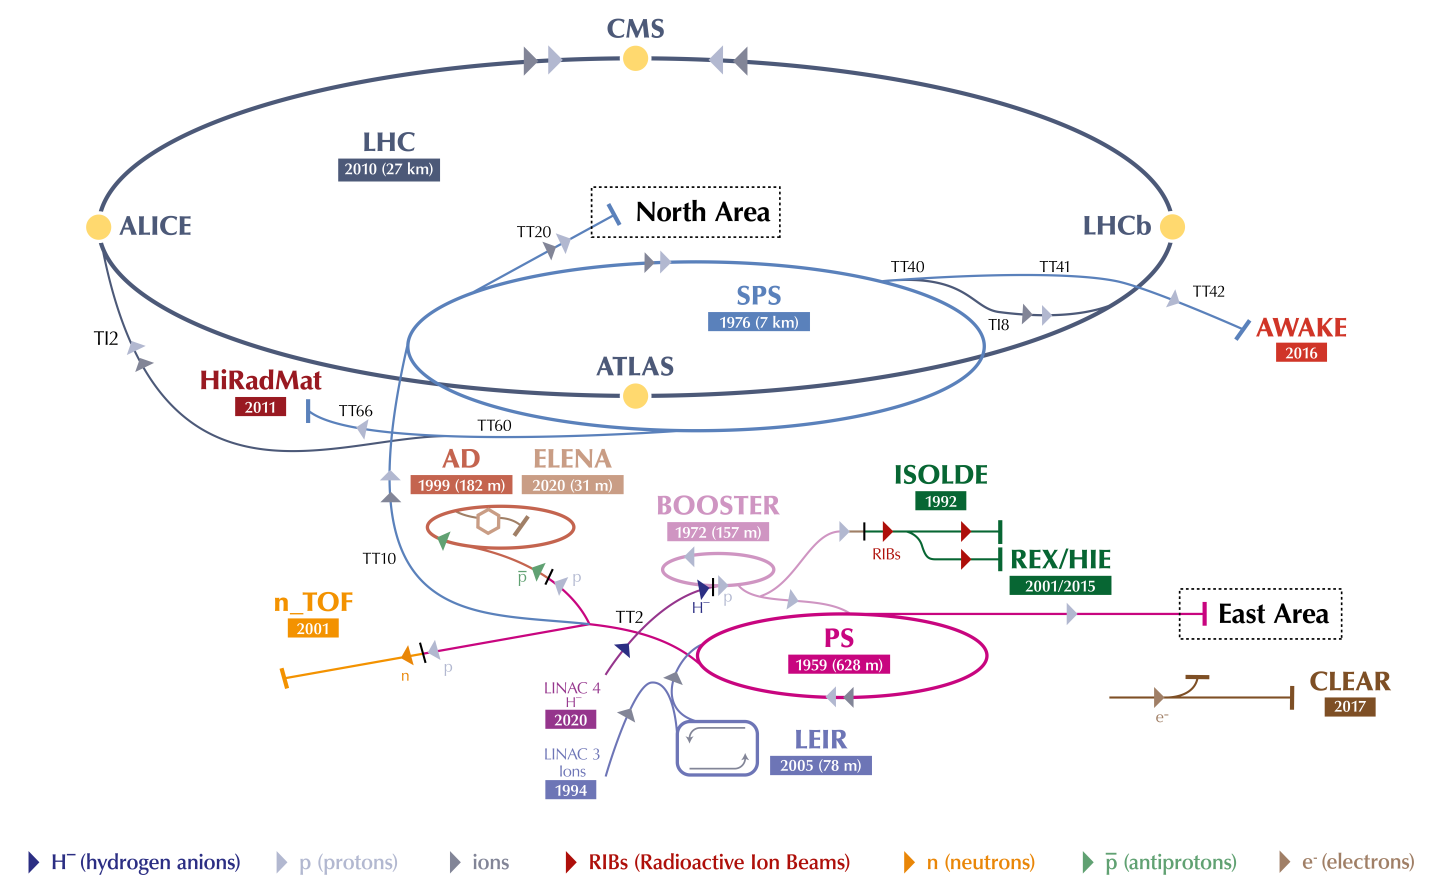
\includegraphics[width=0.8\linewidth]{figures/theoryexperiment/CCC-v2019-final-white_cut}
	\caption{The accelerator complex of the LHC, their corresponding construction years and circumferences. Individual stages are shown in different colours, the particle types they accelerate are indicated as arrows. Note that the pre-acceleators do not serve the LHC ring exclusively and the diverging paths lead to other independent experiments. Old tunnels of previous experiments serve as pre-accelerators now in the LHC injection chain. \cite{Mobs:2684277}}
	\label{fig:lhcstructure}
\end{figure}

The four main stages of pre-acceleration for protons are listed in tab. \ref{tab:preaccelerators} below. As proton source, hydrogen is used. The protons are first accelerated in the form of H$^-$ ions through the 86 metre long tunnel of the recently (2020) constructed Linear Accelerator 4 (Linac4). Stripped of their pair of electrons, the protons enter the Proton Synchrotron Booster (PSB) where they reach up to \SI{2}{\giga\electronvolt}. In the next step of the injection chain, they enter the Proton Synchrotron (PS), historically the first synchrotron at CERN serving exclusively as a pre-accelerator now. Travelling through the 628 metres long ring and accelerated to 26 GeV, the particles are injected into the Super Proton Synchrotron (SPS), where they are awaiting injection into the LHC once they reach 450 GeV.

%https://home.cern/science/accelerators/linear-accelerator-4
%https://home.cern/science/accelerators/proton-synchrotron-booster
%https://home.cern/science/accelerators/proton-synchrotron
%https://home.cern/science/accelerators/super-proton-synchrotron
%https://home.cern/science/accelerators/large-hadron-collider

\begin{table}[h!]
	\centering
	\begin{tabular}{c|c}
		Accelerator & Peak Energy \\
		\hline
		\hline
		Linear accelerator 4 (Linac4) & 160 MeV \\
		\hline
		Proton Synchrotron Booster (PSB) & 2 GeV \\
		\hline
		Proton Synchrotron (PS) & 26 GeV \\
		\hline
		Super Proton Synchrotron (SPS) & 450 GeV \\
		\hline
		Large Hadron Collider (LHC) & 7 TeV \\
	\end{tabular}
	\caption{The acceleration chain the protons undergo to reach their final energy of 7 TeV.}
	\label{tab:preaccelerators}
\end{table}

In the LHC the beams are circulating in opposing directions. They are kept on a circular trajectory using superconducting NbTi magnets operating at \SI{1.9}{\kelvin} thanks to the superfluid helium bath at about \SI{0.13}{\mega\pascal} \cite{Bruning:782076}. In the tunnel itself there are eight interactions points (IP). ATLAS, ALICE, CMS and LHCb are located at IP1, IP2, IP5 and IP8, respectively. IP3 and IP7 are where the momentum and betatron collimators are located ensuring beam quality; the radiofrequency (RF) cavities are at IP4 increasing the bunch energy to 7 TeV. The beam dump is at IP6 where old bunches are deflected by the fast-pulsing "kicker" magnets and directed towards the carbon absorber at the end of their lifetime. \cite{Evans_2008}

\begin{figure}[h!]
	\centering
	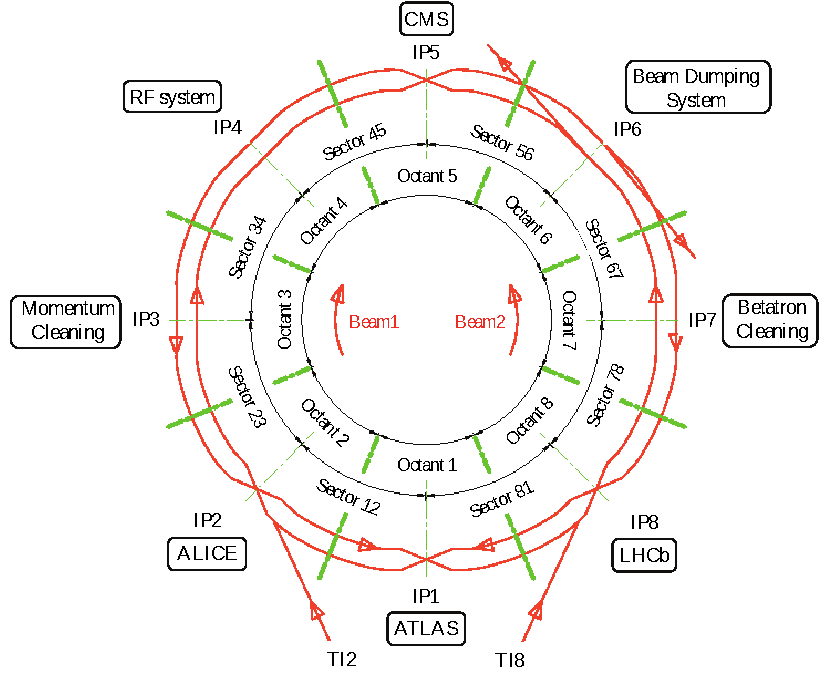
\includegraphics[width=0.6\linewidth]{figures/theoryexperiment/LHC_ring.pdf}
	\caption{The location of the interaction points, the experiments, and the beam adjustment systems. The LHC ring is also divided into further sectors and octants for each IP. \cite{Bracco:1174254}}
	\label{fig:LHC_ring}
\end{figure}

The four main detectors perform the particle collision measurements. LHCb specializes on flavour physics and measures b-quark decays focussing on the measurement and study of CP-violating processes. ALICE has been constructed to mainly study the quark-gluon plasma resulting from heavy ion collisions. ATLAS and CMS are sister experiments and are general purpose detectors. In the following, the latter will be described in detail only.

\Subsection{The Compact Muon Solenoid}

The Compact Muon Solenoid (CMS) detector is a 14 000 tonnes heavy detector measuring 28.7 metres in lenght and 15.9 metres in diameters. It has been built to be general purpose detector, featuring additional muon chambers at its most outer side allowing the precise measurement of muon momenta. The detector is built around a solenoid magnet, producing a magnetic field of $\SI{4}{\tesla}$. CMS has several subdetector components which surround the beampipe in a layered, onion-like structure. CMS has rotational symmetry around the beam pipe along which the z-axis is usually defined. The positions of each components and some of their most important technical details are shown in fig. \ref{fig:cms_view}.

\begin{figure}[h!]
	\centering
	\includegraphics[width=0.8\linewidth]{figures/theoryexperiment/cms_160312_02.pdf}
	\caption{The inner structure of the CMS detector. Note the layered structure and rotational symmetry of the detector. Each layer performs an individual step in particle identification. \cite{Sakuma:2665537}}
	\label{fig:cms_view}
\end{figure}

The coordinate system has its origin at the interaction point, is right-handed, with the $z$-axis pointing towards the anti-clockwise beam direction. Hence, the $xy$ plane lies orthogonal to the beam pipe. Instead of the polar angle directly the pseudorapidity 

\begin{equation*}
	\eta = -\ln\tan\frac{\theta}{2}
\end{equation*}

is used, as it is an Lorentz-invariant quantity along the beam. $\eta = \pm\infty$ hence corresponds to the beampipe and $\eta = 0$ defines the $xy$ (transversal) plane. Using the pseudorapidity, the differences in the $\eta-\phi$ plane can be given by

\begin{equation*}
	\Delta R = \sqrt{\left(\Delta\eta\right)^2 + \left(\Delta\phi\right)^2}
\end{equation*}

With that, particle kinematics can be described in terms of their energy $E$, the transversal momentum $p_T$, $\eta$, $\phi$ and their mass $m$. In some cases, instead of the pseudorapidity, the rapidity

\begin{equation*}
	y = \frac{1}{2}\ln\frac{E+p_z}{E-p_z}
\end{equation*}

is used.

In the following, the main subdetector components, their location and role focussing on high $p_T$ events will be briefly described.

\Subsubsection{Silicon Tracking}

CMS has an all-silicon tracking system, which lies at the core of the detector close to the beam pipe. As the name suggests, the tracking system enables the reconstruction of the trajectories of the child particles passing through the detector. It thus plays a crucial role in particle identification as the charge of particles can be inferred from the track signature (or the lack thereof); apart from that, it also enables secondary vertex reconstruction of short-living primary particles. Particles passing through the silicon ionize the tracker, producing a signal.

Having a length of 5.4 metres and a diameter of 2.4 metres it covers the pseudorapidity range $|\eta|<2.5$, the best tracking efficiency being in the barrel region $|\eta| < 0.9$ \cite{Veszpremi_2014}. Closest to the interaction point lies the pixel silicon tracker. Made-up of four cylindrical layers at $\SI{3}{\centi\meter}$, $\SI{7}{\centi\meter}$, $\SI{11}{\centi\meter}$ and $\SI{16}{\centi\meter}$ from the beam pipe at disks at the end, it is segmented into 124 million pixels of $\SI{100}{\micro\meter} \times \SI{150}{\micro\meter}$ and kept at $\SI{-20}{\degreeCelsius}$ during operation.

Outside of the silicon pixel detector lie the silicon strip detectors, which is divided into four parts: the inner barrel par (TIB), the inner disk part (TID), the outer barrel (TOB) and the outer endcap part (TEC). This part of the tracker contains about 10 million strip components. The complete layout of the strip detectors is shown in fig. \ref{fig:strip_tracker}.

\begin{figure}[h!]
	\centering
	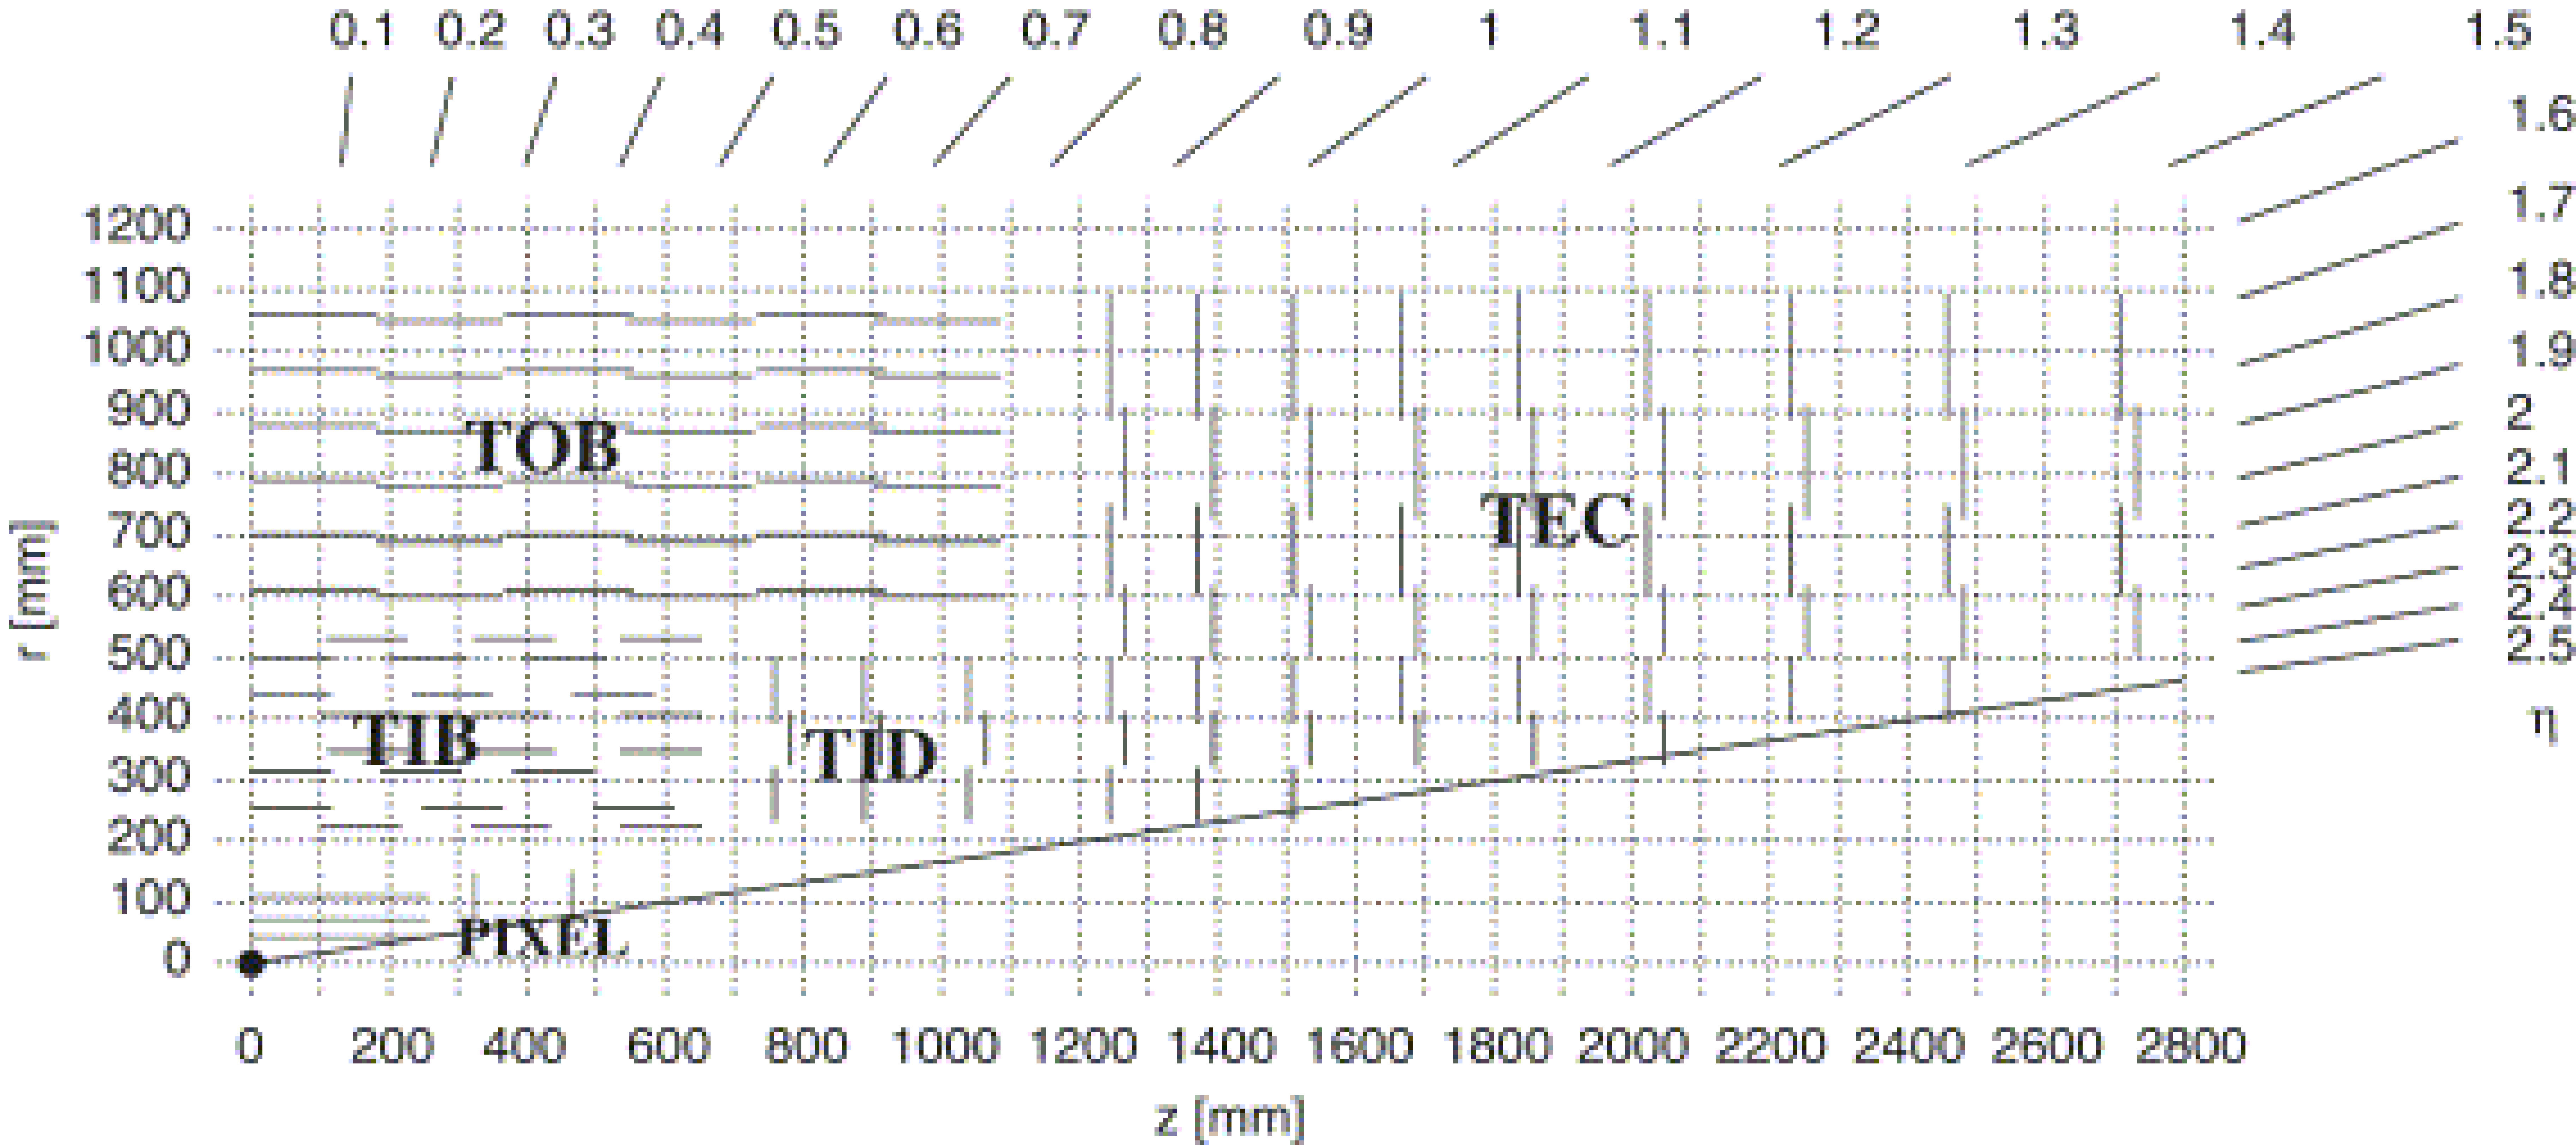
\includegraphics[width=0.8\linewidth]{figures/theoryexperiment/StripTracker}
	\caption{View of one quarter of the silicon strip detectors in the $r-z$ plane, indicating both the geometry and the pseudorapidity range of the individual parts. \cite{Azzurri:914891}}
	\label{fig:strip_tracker}
\end{figure}

\Subsubsection{Electromagnetic Calorimeter}

The CMS electromagnetic calorimeter (ECAL) measures the energy of electrons and photons by absorbing them completely and measuring the induced particle shower during that. It lies outside of the tracking system and consists of highly transparent and scintillating lead tungstate (PbWO$_4$) crystals. The ECAL consists of two components as well, and central barrel (EB) covering the region up to $|\eta| = 1.48$ and an endcap region (EE) extending this coverage to pseudorapidities of $|\eta| = 3.0$ \cite{Biino_2015}. The EB has 61 200 crystals, which are formed into modules weighing around $\SI{3}{\tonne}$ and containing 1700 crystals, which are $\SI{23}{\centi\meter}$ (or $25.8 X_0$ in terms of radiation length $X_0$) in length. The EC and the end of the barrel modules have almost 15 000 more crystals; the total volume of the crystals is $\SI{11}{\cubic\meter}$ with a weight of $\SI{92}{\tonne}$. The layout of the calorimeter structure is shown in fig. \ref{fig:ecal}.

\begin{figure}[h!]
	\centering
	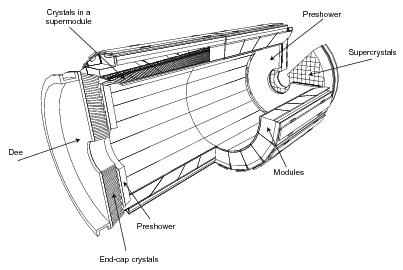
\includegraphics[width=0.6\linewidth]{figures/theoryexperiment/ecal.png}
	\caption{Schematic view of the CMS barrel and endcap calorimeters. Note the coverage around the tracker (not shown explicitly) and the preshower module, responsible for better seperation of photon hits in the endcap region. \cite{Chatrchyan:1554142}}
	\label{fig:ecal}
\end{figure}

The energy resolution of the barrel calorimeters has tree terms: a stochastic, a noise and a constant term and was measured to be \cite{Chatrchyan:1554142}

\begin{equation*}
	\frac{\sigma_E}{E} = \underbrace{\frac{2.8\%}{\sqrt{E(GeV)}}}_\text{stochastic} \oplus \, \underbrace{\vphantom{\frac{2.8\%}{\sqrt{E(GeV)}}}\frac{12\%}{E(GeV)}}_\text{noise} \oplus \, \underbrace{\vphantom{\frac{2.8\%}{\sqrt{E(GeV)}}}0.3\%}_\text{constant}
\end{equation*}

%In the barrel region the crystals are equipped with avalanche photodiodes (APD) of $5 \times \SI{5}{\square\milli\meter}$ and they are insensitive to the $\SI{4}{\tesla}$ magnetic field in the detector.

\Subsubsection{Hadronic Calorimeter}

The CMS hadronic calorimeters (HCAL) is a sampling calorimeter. Similarly to the ECAL, its purpose is to measure the energy of hadrons by measuring the induced avalanche of secondary particles upon passing through the detector as they are not directly stopped in the ECAL. In the $|\eta|<3$ region it consists of a brass scintillator calorimeter; in the forward region $3<|\eta|<5$ in has a iron quartz-fiber calorimeter \cite{canko_ak_2009}. It is organized into barrel (HB), outer barrel (HO), endcap (HE) and forward (HF) regions. The layout and the positioning of the respective components are shown in fig. \ref{fig:hcal}.

\begin{figure}[h!]
	\centering
	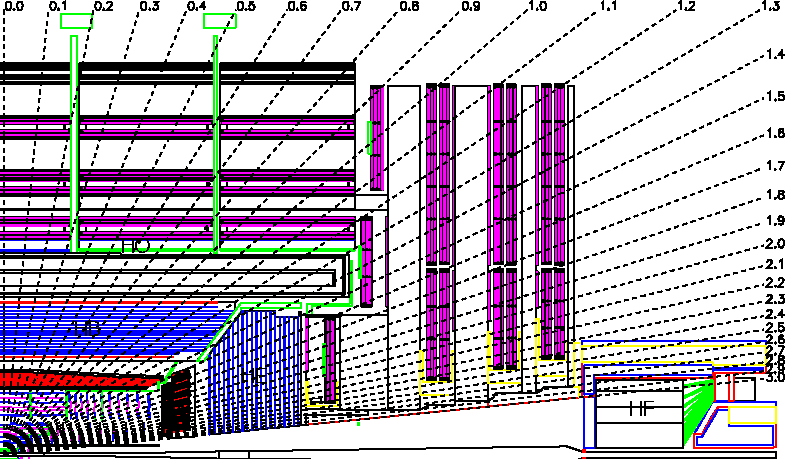
\includegraphics[width=0.8\linewidth]{figures/theoryexperiment/hcal.pdf}
	\caption{The CMS HCAL module setup. Note that the outer calorimeter lies outside of the solenoid (the white rectangle between HB and HO). \cite{Chatrchyan:1129810}}
	\label{fig:hcal}
\end{figure}

\Subsubsection{Superconducting Solenoid Magnet and the Return Yokes}

A core component of the detector is the solenoid magnet itself. Weighing $\SI{12000}{\tonne}$ and cooled down to $\SI{-268.5}{\degreeCelsius}$ it can produce a magnetic field of $\SI{4}{\tesla}$ ($\SI{3.8}{\tesla}$ during the runs), it is the largest solenoid in the world. The solenoid magnet and the return yokes play a crucial role in particle identification and muon measurement. These high magnetic fields are achieved using NbTi coils and a current of $\SI{18160}{\ampere}$. Outside of the solenoid magnet itself lie the muon chambers and the five return yokes, which are constructed from steel. The field strength thanks to the yokes there is around $\SI{2}{\tesla}$.

\Subsubsection{Muon Chambers}

In the outermost layers of the detector, the muon chambers can be found. CMS specializes in muon measurements and these chambers are characteristic for the whole detector. As muons provide a clear signature (like in a $H \rightarrow ZZ \rightarrow \mu\mu\mu\mu$, which is referred to as the "Golden Channel"), their reconstruction is highly motivated. Due to muons having several orders of magnitude higher mass compared to electrons, they can pass the ECAL and they are not stopped there.  Hence, they do not deposit their complete energy there meaning they can escape all the inner detector components. For this reason, additional measurements on their momenta are needed.

The chambers have four subcomponents: the drift tubes (TB), the cathode strip chambers (CSCs), the resistive plate chambers (RPCs) and the gas electron multipliers (GEMs), all of which are gaseous detectors. In the region $|\eta|<1.2$ the four layers of drift tubes have been installed at a radius of approximately $\SI{4}{\meter}$, $\SI{4.9}{\meter}$, $\SI{5.9}{\meter}$ and $\SI{7}{\meter}$. The tubes consist of 250 chambers and looking from the transversal plane, they are grouped into 12 sectors, with each covering 30° azimuthal angle. These chambers are staggered in a way, such that a high $p_T$ muon produced a the sector boundary crosses at least 3 of the four layers. In the endcap region up to $|\eta| < 2.4$, the CSCs are deployed. The CSCs are used both in the endcap and the barrel region. The newly added GEMs have been installed in the region $1.6 < |\eta| < 2.2$ \cite{Colaleo:2021453}. The exact position of the components are shown in fig. \ref{fig:muonchambers}.

\begin{figure}[h!]
	\centering
	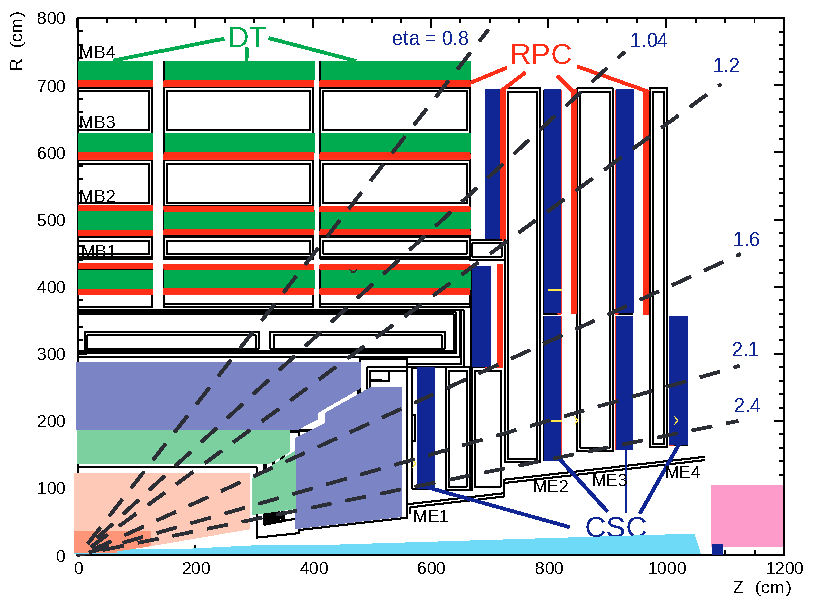
\includegraphics[width=0.8\linewidth]{figures/theoryexperiment/muonchambers.pdf}
	\caption{The location of the drift tubes (DT), the cathode strip chambers (CSCs) the resistive plate chambers (RPCs). The newly deployed GEMs are in the region $1.6 < |\eta| < 2.2$ (not shown here) \cite{Bayatian:922757}.}
	\label{fig:muonchambers}
\end{figure}

\Subsubsection{Trigger System}

With a collision frequency of $\SI{40}{\mega\hertz}$ with a new collision in every $\SI{25}{\nano\second}$ it is impossible to record every event in the detector.

\begin{figure}[h!]
	\centering
	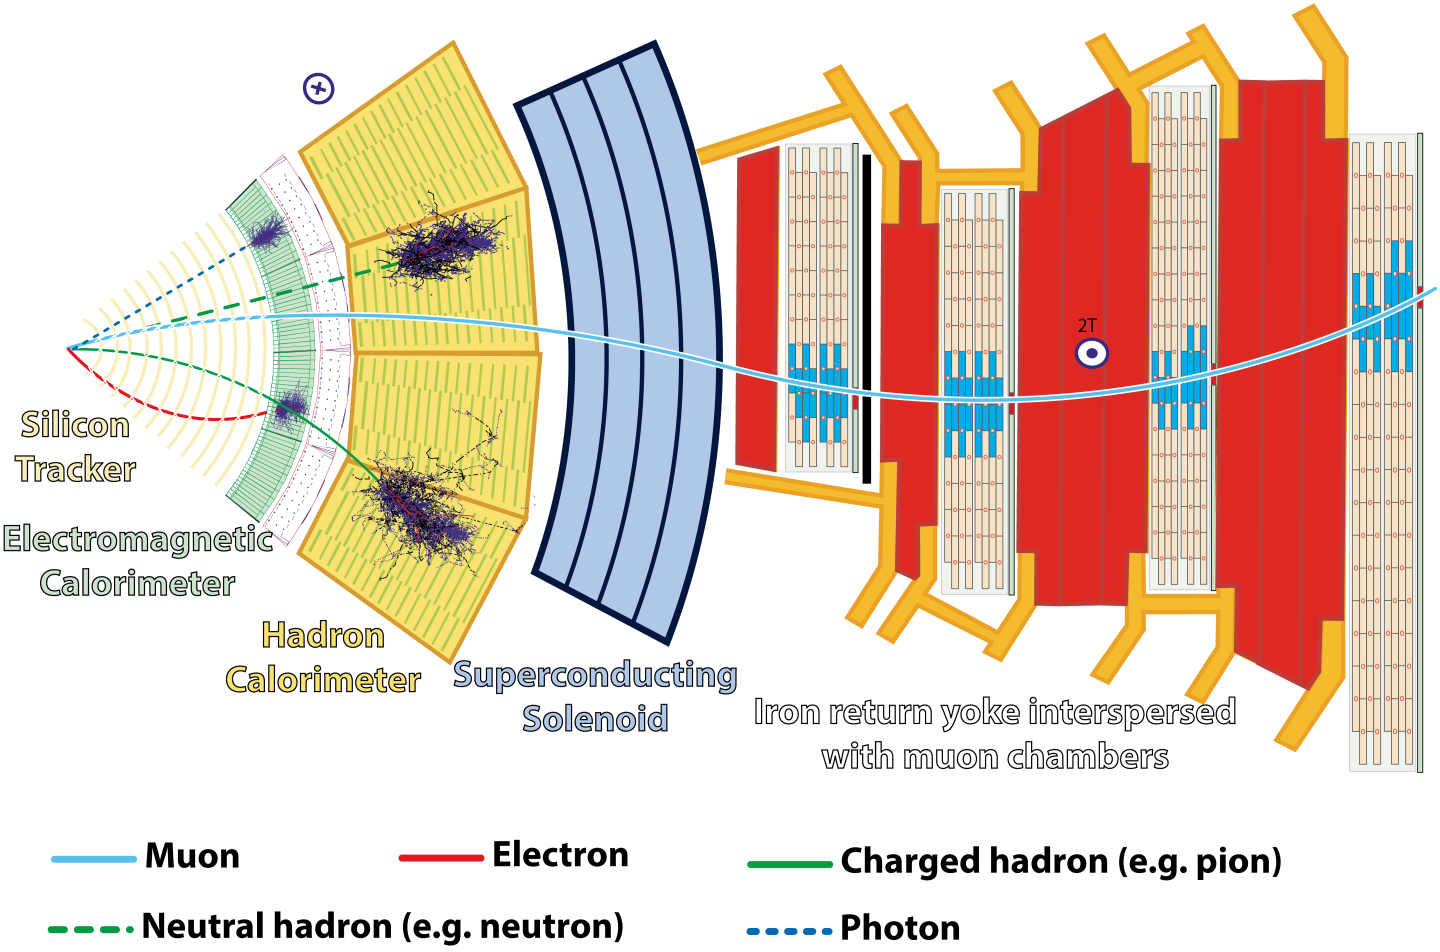
\includegraphics[width=0.8\linewidth]{figures/theoryexperiment/CMS_Slice}
	\caption{from \cite{Barney:2120661}}
	\label{fig:cms_slice}
\end{figure}